\chapter{Fields}
\label{chapter:Fields}
\thispagestyle{empty}


In Chapter~\ref{chapter:PolyEquations}, we explored problems about finding and expressing roots of polynomials, finally arriving at the goal of the course: proving that there are quintic polynomials that are \emph{not} solvable by radicals. This chapter serves two main purposes. First, as we look at roots of polynomials and how they can be expressed, it will be convenient to have a common world (i.e.~number system) in which they live. For us, this will be the complex numbers, denoted $\mathbb{C}$, which will be reviewed below. Our work with complex numbers will also supply the necessary language to properly talk about $n^{\text{th}}$-roots. Second, we are still in need of a proper definition of what it means for a polynomial to be ``solvable by radicals''; this is where the chapter will finish. But the middle of the chapter is perhaps the most interesting. There, on the way to defining ``solvable by radicals'', we will be led to abstract the structure of $\mathbb{C}$ (and of $\mathbb{Q}$ and $\mathbb{R}$), arriving at the definition of a \emph{field}. 

\begin{section}{Complex Numbers}
As mentioned above, we want to work in a world that contains all of the roots of all of the polynomials that we will be studying. Considering the roots of polynomials such as $x^2 +1$, $x^2-2$, $x^2-3$, etc., we see that we need to include numbers like $\sqrt{-1}$, $\sqrt{2}$, $\sqrt{3}$, etc., so although there are smaller worlds one could choose, we will opt for the world containing both $\sqrt{-1}$ and $\mathbb{R}$, namely $\mathbb{C}$.

But before we proceed, note that $\sqrt{-1}$ is not really well defined. There are \emph{two} solutions to $x^2 +1$, so when we write $\sqrt{-1}$, we are all agreeing that we mean the same one. 

\begin{definition}
Let $i$ (or alternatively $\sqrt{-1}$) denote one particular solution to $x^2 +1$. 
\end{definition}

Of course, the previous definition implies that $i^2 = -1$. Using $i$ and $\mathbb{R}$, we now build the complex numbers.

\begin{definition}
The \textbf{complex numbers} is the set $\mathbb{C} := \{a + bi\mid a,b \in \mathbb{R}\}$. If $z=a+bi$, then $a$ is called the \textbf{real part} of $z$ and $b$ is called the \textbf{imaginary part} of $z$.
\end{definition}

Note that every complex number $z=a+bi$ is uniquely determined by two numbers: the real and imaginary parts $a$ and $b$. As such, we often graph complex numbers in the coordinate plane with the $x$-axis denoting the real part and the $y$-axis denoting the imaginary part. This will be called the \textbf{complex plane}.

\begin{example}
We graph $-2 + 2i$ and  $1 - 3i$ below.
\begin{center}
\begin{tikzpicture}[line width = .9,scale = .7]
\draw[<->] (-4,0) -- (4,0) node [below] {\small \textsc{Real}};
\draw[<->] (0,-4) -- (0,4) node [left] {\small \textsc{Imag.}};
\foreach \i in {1,2,3} {
\draw (-\i,-0.1) -- (-\i,0.1);
\draw (\i,-0.1) -- (\i,0.1);
\node[anchor = 90] at (-\i,0) {\small $\i$};
\node[anchor = 90] at (\i,0) {\small $\i$};
\draw (-0.1,-\i) -- (0.1,-\i);
\draw (-0.1,\i) -- (0.1,\i);
\node[anchor = 0] at (0,-\i) {\small $\i$};
\node[anchor = 0] at (0,\i) {\small $\i$};
}
\node (w) at (-2,2) {};
\fill (w) circle (.1);
\node[anchor = -10] at (w) {\small $-2 + 2i$};
\node (z) at (1,-3) {};
\fill (z) circle (.1);
\node[anchor = 170] at (z) {\small $1 - 3i$};
\end{tikzpicture}
\end{center}
\end{example}

We also define some operations on complex numbers.

\begin{definition}
We define the following operations on elements of $\mathbb{C}$. 
\begin{itemize}
\item \textbf{Addition:} $(a+bi) + (c+di) := (a+b) + (c+d)i$
\item \textbf{Multiplication:} $(a+bi) \cdot (c+di) := (ac-bd) + (ad+bc)i$
\item \textbf{Complex Conjugation:} $\overline{a+bi} := a-bi$
\end{itemize}
\end{definition}

Notice that in the definition of complex multiplication we are just using the normal distributive law (or FOIL if you like) together with the fact that $i^2 = -1$. Many of the familiar algebraic properties of $\mathbb{R}$ also hold for $\mathbb{C}$, which we will take as a fact.

\begin{fact}\label{fact.ComplexLaws} The following are true for $\mathbb{C}$.
\begin{itemize}
\item \textbf{Addition Laws:} Addition is associative and commutative. There is a unique additive identity, namely $0 = 0 + 0i$, and every number has a unique additive inverse, denoted $-(a+bi)$.
\item \textbf{Multiplication Laws:} Multiplication is associative and commutative. There is a unique multiplicative identity, namely $1 = 1 + 0i$, and every nonzero number has a unique multiplicative inverse, denote $(a+bi)^{-1}$ or $\frac{1}{a+bi}$.
\item \textbf{Distributivity Laws:} For all $a,b,c \in \mathbb{C}$, $a(b+c) = ab+ac$ and $(b+c)a = ba+ca$.
\item \textbf{Conjugation Laws:} For all $a,b \in \mathbb{C}$, $\overline{a+b} = \overline{a} + \overline{b}$ and $\overline{ab} = \overline{a}\overline{b}$.
\end{itemize}
\end{fact}

\begin{problem}
Thinking of a complex number $z$ as a point in the complex plane, describe \emph{geometrically} what happens when $(c+di)$ is added to $z$. Also, describe \emph{geometrically}  how to find $\overline{z}$ from $z$.
\end{problem}

When we plot points, there are different coordinate systems we could use. It turns out that  rectangular coordinates are good for adding complex numbers, but polar coordinates are better for multiplication. This lead to the following definition.

\begin{definition}
Let $z=a+bi$. 
\begin{enumerate}
\item The \textbf{modulus} of $z$, denoted $|z|$, is the radius of the point $(a,b)$ when written in polar coordinates. Thus, $|z| = \sqrt{a^2 + b^2}$. 
\item The \textbf{argument} of $z$, denoted $\Arg(z)$, is the angle of the point $(a,b)$ when written in polar coordinates. Thus, $\Arg(z)$ is the angle $\theta$ \emph{in the appropriate quadrant} such that $0\le \theta<2\pi$ and $\tan \theta = \frac{b}{a}$. The argument of  $0$ is undefined.
\end{enumerate}
\end{definition}

\begin{example}
We have that $|-2 + 2i| = \sqrt{(-2)^2+2^2} = 2\sqrt{2}$ and $\Arg(-2 + 2i) = \frac{3\pi}{4}$. (But be careful, $\arctan\left(\frac{2}{-2}\right) = \frac{\pi}{4}$; you must pay attention to which quadrant the number is in.)
\begin{center}
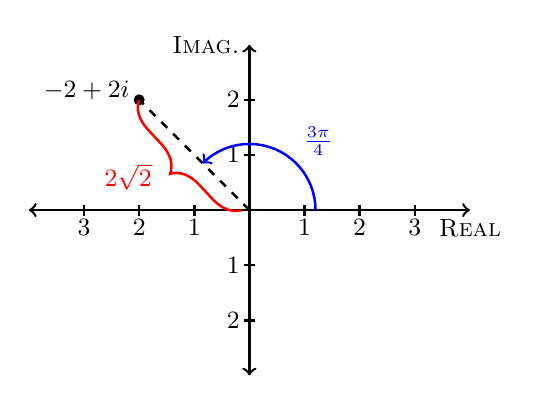
\begin{tikzpicture}[line width = .9,scale = .7]
\small
\draw[<->] (-4,0) -- (4,0) node [below] { \textsc{Real}};
\draw[<->] (0,-3) -- (0,3) node [left] { \textsc{Imag.}};
\foreach \i in {1,2,3} {
\draw (-\i,-0.1) -- (-\i,0.1);
\draw (\i,-0.1) -- (\i,0.1);
\node[anchor = 90] at (-\i,0) { $\i$};
\node[anchor = 90] at (\i,0) { $\i$};
}
\foreach \i in {1,2} {
\draw (-0.1,-\i) -- (0.1,-\i);
\draw (-0.1,\i) -- (0.1,\i);
\node[anchor = 0] at (0,-\i) { $\i$};
\node[anchor = 0] at (0,\i) { $\i$};
}
\node (w) at (-2,2) {};
\fill (w) circle (.1);
\node[anchor = -10] at (w) { $-2 + 2i$};

\draw [dashed] (0,0) -- (w.center);
\draw [blue,domain=0:135,->] plot ({1.2*cos(\x)}, {1.2*sin(\x)});
\node[blue] at (1.25,1.25) {$\frac{3\pi}{4}$};

\draw [red,decorate,decoration={brace,amplitude=10pt},xshift=-4pt,yshift=0pt]
(0,0) -- (w.center);
\node[red] at (-2.2,0.6) {$2\sqrt{2}$}; 
\end{tikzpicture}
\end{center}
\end{example}

\begin{problem}\label{prob.ComplexCheckin}
For each of the following complex numbers,
\begin{itemize}
\item write it in the form $a+bi$ (if it is not already),
\item plot it in the complex plane,
\item find the modulus and argument (if not exact, then a decimal approximation is okay).
\end{itemize}
\begin{multicols}{2}
\begin{enumerate}
\item $u = -1-i$
\item $v= \frac{1}{1+i}$
\item $w = \frac{(2-i)(1+2i)}{2+3i}$
\item $z\in \mathbb{C}$ with $|z| = 3$ and $\Arg(z) = \frac{4\pi}{3}$
\end{enumerate}
\end{multicols}
\end{problem}

\begin{theorem}
Let $z\in \mathbb{C}$. If $z\neq 0$, then $z^{-1} = \displaystyle\frac{\overline{z}}{|z|}$.
\end{theorem}

The next theorem shows how to find an expression for a complex number given its modulus and argument.
 
\begin{theorem}\label{thm.PolarToRectangular}
Let $z\in \mathbb{C}$. Then $|z| = r$ and $\Arg(z) = \theta$ if and only if $z = r\cos\theta + ir\sin\theta$ with $0\le \theta <2\pi$.
\end{theorem}

We now derive some properties of multiplication. The first is quite useful and illustrates how multiplication is rather easy to deal with when numbers are in ``polar form''.

\begin{theorem}\label{thm.MultiplyComplex}
If $z_1 = r_1\cos\theta_1 + ir_1\sin\theta_1$ and $z_2=r_2\cos\theta_2 + ir_2\sin\theta_2$, then \[z_1z_2 = r_1r_2\cos(\theta_1+\theta_2) + ir_1r_2\sin(\theta_1+\theta_2).\]
\end{theorem}

\begin{corollary}
If $z_1,z_2\in \mathbb{C}$, then $|z_1z_2| = |z_1||z_2|$ and $\Arg(z_1z_2) = \Arg(z_1)+\Arg(z_2)$.
\end{corollary}

\begin{corollary}[De Moivre's formula]\label{cor.DeMoivre}
For each positive $n\in \mathbb{Z}$, \[\left(r\cos(\theta) + ir\sin(\theta)\right)^n = r^n\cos(n\theta) + ir^n\sin(n\theta).\]
\end{corollary}

We now arrive at an \emph{extremely important} definition.

\begin{definition}
For each positive $n\in \mathbb{Z}$, define \[\zeta_n := \cos\left(\frac{2\pi}{n}\right) + i\sin\left(\frac{2\pi}{n}\right).\]
Thus, $\zeta_n$ (read as ``zeta n'') is the unique  number with magnitude $1$ and argument $\frac{2\pi}{n}$.
\end{definition}

\begin{problem}
Plot each of the following in the same complex plane: $\zeta_2$, $\zeta_3$, $\zeta_4$, $\zeta_5$.
\end{problem}

\begin{problem}
Plot each of the following in the same complex plane: $\zeta_6$, $(\zeta_6)^2$, $(\zeta_6)^3$, $(\zeta_6)^4$, $(\zeta_6)^5$, $(\zeta_6)^6$.
\end{problem}

\begin{problem}
Write $\overline{\zeta_8}$ as a power of $\zeta_8$. Conjecture and prove a formula that expresses $\overline{(\zeta_n)^k}$ as a power of $\zeta_n$, but with no bar on top.
\end{problem}

We now turn our attention back to solving polynomial equations, focusing on those of the form $x^n - a$.

\begin{definition}
Let $a\in \mathbb{C}$. A number $z\in \mathbb{C}$ is called an \textbf{$n^\text{th}$ root of $a$} if $z^n = a$. In other words, the  $n^\text{th}$ roots of $a$ are the roots of the polynomial $x^n-a$. The  $n^\text{th}$ roots of $1$ are also called \textbf{$n^\text{th}$ roots of unity}.
\end{definition}

\begin{problem}
Find a $4^\text{th}$ root of each of the following: $\zeta_3$ and $-1 + i\sqrt{3}$.
\end{problem}

\begin{theorem}
For each non-negative $k\in \mathbb{Z}$, $(\zeta_n)^k$ is an $n^\text{th}$ root of $1$.
\end{theorem}

\begin{lemma}\label{lem.nthRoot1IsPowerOfZeta}
If $z$ is an $n^\text{th}$ root of $1$, then $z = (\zeta_n)^k$ for some non-negative $k\in \mathbb{Z}$.
\end{lemma}

\begin{lemma}
For each non-negative $k\in \mathbb{Z}$, $(\zeta_n)^k = (\zeta_n)^m$ for some $0\le m \le n-1$.
\end{lemma}

\begin{theorem}\label{thm.nthRoots1}
The set \[\{1, \zeta_n, (\zeta_n)^2, \ldots, (\zeta_n)^{n-1}\}\] is the set of \emph{all} $n^\text{th}$ roots of unity. Thus, there are $n$ distinct $n^\text{th}$ roots of unity. 
\end{theorem}

\begin{lemma}
Let $a\in \mathbb{C}$ be nonzero, and let $b$ be any one particular $n^\text{th}$ root of $a$. Then $z$ is an $n^\text{th}$ root of $a$ if and only if $\frac{z}{b}$ is an $n^\text{th}$ root of $1$.
\end{lemma}

\begin{theorem}\label{thm.nthRoots}
Let $a\in \mathbb{C}$ be nonzero, and let $b$ be any one particular $n^\text{th}$ root of $a$. The set \[\{b, b\zeta_n, b(\zeta_n)^2, \ldots, b(\zeta_n)^{n-1}\}\] is the set of \emph{all} $n^\text{th}$ roots of $a$. Thus, there are $n$ distinct $n^\text{th}$ roots of $a$. 
\end{theorem}

\begin{problem}
Find \emph{all} $4^\text{th}$ roots of each of the following: $\zeta_3$ and $-1 + i\sqrt{3}$.
\end{problem}


We conclude this section with a couple of general results about roots of polynomials.

\begin{theorem}\label{thm.RootsRealCoeff}
Suppose that $p(x) = a_nx^n + a_{n-1}x^{n-1} +\cdots+a_2x^2+a_1x+a_0$ with all $a_i\in \mathbb{R}$. If $z$ is a root of $p(x)$, then $\overline{z}$ is also a root of $p(x)$.
\end{theorem}

In words, the previous theorem says that if a polynomial has coefficients in $\mathbb{R}$, then the set of roots is ``closed under complex conjugation.'' We end with an extremely important theorem, which will be quite useful for us. However, since its proof is not our main goal (and since it requires sophisticated techniques), we will take it as fact.

\begin{fact}[Fundamental Theorem of Algebra]
If $p(x)$ is a non-constant polynomial with all coefficients in $\mathbb{C}$, then $p(x)$ has a root in $\mathbb{C}$.
\end{fact}

In fact, we will see that this implies that \emph{all} roots of such a $p(x)$ lie in $\mathbb{C}$, so in our of study polynomials (often with all coefficients even in $\mathbb{Q}$), $\mathbb{C}$ serves as a uniform world in which we can study the roots.
\end{section}

\begin{section}{An aside: the Quaternions}


\end{section}



% Don't forget hamiltonians







